\documentclass[aps,prl,reprint]{revtex4-1}
\usepackage{blindtext}

\usepackage{amsmath}
\usepackage{graphicx}
\usepackage{commath}
\usepackage{siunitx}
\usepackage{tabularx}
\usepackage{subcaption}

\usepackage{amssymb}

\usepackage{float}

\usepackage{graphicx}


\usepackage[b]{esvect}


\newcommand{\de}{\mathrm{d}}
\newcommand{\vcc}{V_\text{CC}}
\newcommand{\parallelsum}{\mathbin{\!/\mkern-5mu/\!}}


\graphicspath{ {images/} }
\begin{document}

\title{Unit 6: Elements of Digital Electronics}
\author{Xueqi Li}
% \email{xueqi.li@stonybrook.edu}
\thanks{Partner: Tianming Hai}
\noaffiliation
\date{Apr 28, 2018}


% \begin{abstract}
% In this lab we introduced operational amplifier and the negative feedback. Furthermore, a few importent applications of amplifier, such as follower, inverting and non-inverting amplifier, integrator, and differentiator were discussed and their output voltage formulas have been derived. Moreover, the limit of the opamp was explored and two methods to measure the slew rate have been given as examples.
% \end{abstract}

\maketitle

\section{Introduction}  
	\subsection{Binary}
		To change a number to binary or to convert back to decimal, one can use following equation:
        \begin{align}
            &(B_n B_{n-1} \cdots B_2 B_1 B_0)_2 \\ \nonumber
            :=& \sum_{i = 0}^n B_i 2^i = \sum_{i = 0}^k D_i 10^i \\ \nonumber
            =:& (D_k D_{k-1} \cdots D_2D_1D_0)_{10} \label{eq:binaryToDecimal}
        \end{align}
        On the other hand, for any base-$n$ to base-$m$ numberal system:
        \begin{align}
            &(N_a N_{a-1} \cdots N_2 N_1 N_0)_2 \\ \nonumber
            :=& \sum_{i = 0}^a N_i n^i = \sum_{i = 0}^b M_i m^i \\ \nonumber
            =:& (M_b M_{b-1} \cdots M_2M_1M_0)_{10} \label{eq:arbitraryConvert}
        \end{align}
        For example, if one wants to convert $(137)_{10}$, using Equation~\ref{eq:binaryToDecimal}, one can find following:
        \begin{align*}
            (137)_{10}& \\
            =& 1\times 10^2 + 3\times 10^1 + 7\times 10^0 \\
            =& 1 \times 2^7 + 1 \times 2^3 + 1 \times 2^0\\
            =& (10001001)_{2}
        \end{align*}
        On the other hand, if one wants to convert $(100101)_2$ to decimal, using Equation~\ref{eq:binaryToDecimal},one can obtain:
        \begin{align*}
            (100101)_2&\\
            =& 1 \times 2^5 + 1\times 2^2 + 1\times 2^0\\
            =& 3 \times 10^1 + 7\times 10^0\\
            =& 37
        \end{align*}
    \subsection{Logic and Truth Table}
        It is well-know that from logic equation to truth table, one can just plug in all possible input, and calculate the output. On the other hand, one may wants to convert a truth table into logic equation. To do so, one can chose each output 1 line from the truth table, and add (or) them up.

        \begin{table}[h]
        \begin{tabular}{ccccc} 
        A&B&X&Y&O \\ \hline
        1&0&0&1&1 \\ 
        1&1&0&1&1 \\ 
        0&0&0&1&0 \\ 
        0&1&0&1&0 \\ 
        0&1&1&0&1 \\ 
        1&1&1&0&1 \\ 
        0&0&1&0&0 \\ 
        1&0&0&0&0 \\ 
        \end{tabular}
        \caption{Truth table of a 2 selector. A,B are input; X,Y are select input}
        \label{table:selector}
        \end{table} 
        For example, a selector have $n$ input, and $\log_2(n)$ select input. The select input select the input to be the output. For example, a 2 selector have truth table as Table~\ref{table:selector}. We can chose the output 1 one and add them, Thus we have
        \[
        O = A \bar B \bar X Y + AB\bar X Y + \bar A B X \bar Y + ABX \bar Y
        \]
    \subsection{Transistor-transistor Logic}
        In TTL system, the binary number can be present as high or low voltage. In ideal case, 0V is low and 5V is high. However, in real world, it is not possible to always obtain a 5V or 0V voltage. Thus, for TTL standard, any input higher than 2V is high, and any input lower than 0.8V is low. On the other hand, any output 3.5V is high and any ouput 0.5V is low.
    \subsection{Logic Gate}
        A logic gate accept some inputs and gives an output. The logic gate's truth table is same as mathematical logic. In the lab, we use NOT, AND, NAND, OR, NOR, XOR, and XNOR gate. The truth table is given in the appendix.

        \begin{figure}[h]
            \centering
            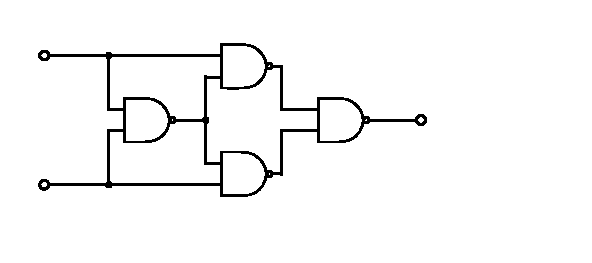
\includegraphics[height=1in]{image/NAND-XOR.pdf}
            \caption{Form a XOR gate using NAND gate}
            \label{fig:nandToXor}
        \end{figure}
        One can use NAND gate to form any other logic gate. For example, Figur~\ref{fig:nandToXor} present how to form a XOR gate from NAND gate. The truth table is in the appendix.
    \subsection{Full-adder}
        \begin{figure}[h]
            \centering
            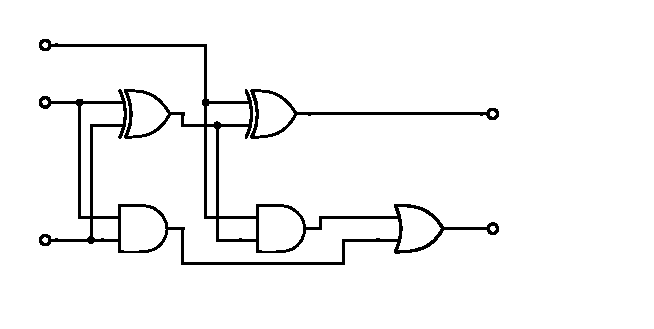
\includegraphics[height=1.5in]{image/Full-Adder.pdf}
            \caption{A full-adder}
            \label{fig:fullAdder}
        \end{figure}
        One importent application of logic gate is full-adder, presented in Figure~\ref{fig:fullAdder}, where the left side is input and the right side is output. The output of a full-adder is the result of binary addition of the input.
        \subsubsection{Two Bit Half-adder}
            \begin{figure}[h]
                \centering
                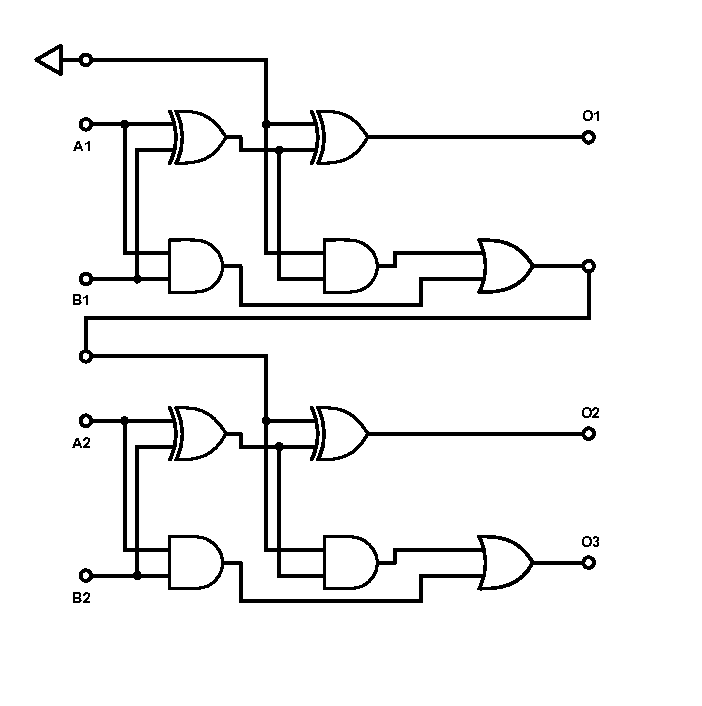
\includegraphics[height=3in]{image/Two-Bit-Half-adder.pdf}
                \caption{A Two Bit Half-adder}
                \label{fig:twoBitHalfAdder}
            \end{figure}
            Once obtain a full-adder, one can use full-adder to form a higher bit adder. For example, one can obtain a two bit half-adder as in Figure~\ref{fig:twoBitHalfAdder}
    \subsection{Flip-flop}
        \begin{figure}[h]
            \centering
            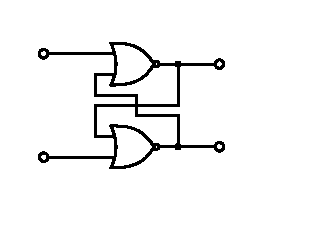
\includegraphics[height=1in]{image/Flip-flop.pdf}
            \caption{A Flip-flop}
            \label{fig:flipFlop}
        \end{figure}
        A Flip-flop, shown in Figure~\ref{fig:flipFlop}, can output one or zern when input are different and hold the output when two ouput are zero. There are a few application of flip-flop.
        \subsubsection{Clocks}
            \begin{figure}[h]
                \centering
                \subcaptionbox{555 Chip}[.49\linewidth][c]{%
                    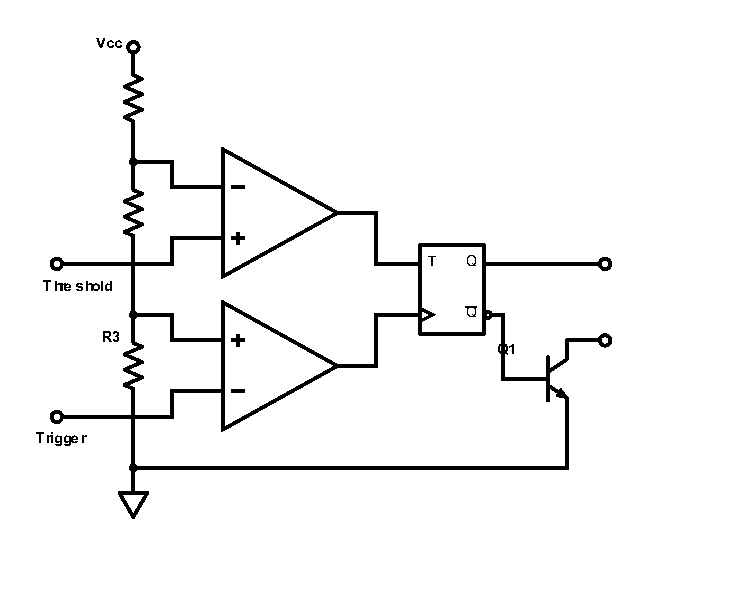
\includegraphics[width=.55\linewidth]{image/555-Chip.pdf}}
                \subcaptionbox{A Clock}[.49\linewidth][c]{%
                    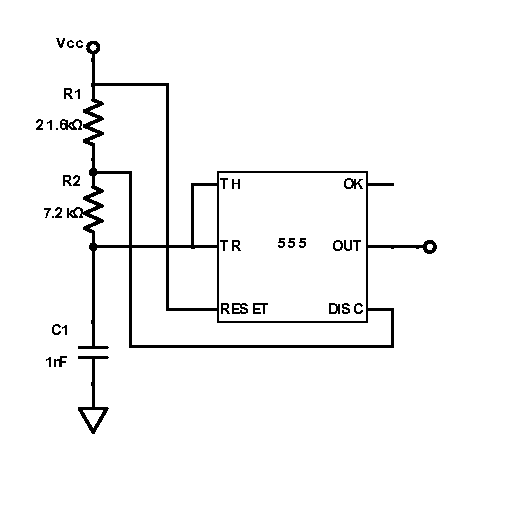
\includegraphics[width=.44\linewidth]{image/Clocks.pdf}}
                \caption{An application of flip-flop}
                \label{fig:clocks}
            \end{figure}
            A nice application of flip-flop is clock. The key of the clock is the 555 chip, which is an application of flip-flop. The circuit of a 555 chip is present in Figure~\ref{fig:clocks}a, where all resistors are 5k$\Omega$. The 555 chip divide $\vcc$ into 3 parts, when trigger voltage is larger than 1/3 $\vcc$ and threshold voltage is smaller than 2/3 $\vcc$, the out put is hold, otherwise it the output is 1 or zero if trigger voltage is below 1/3 $\vcc$ or threshold voltage is higher than 2/3 $\vcc$.

            Than the clock is present in Figure~\ref{fig:clocks}b. This circuit can let the voltage periodically output zero or one, depending on the RC circuit. Thus, using by calculate the voltage in capastor, one can find the period of the circuit.
            \begin{align*}
                V_C &= \vcc (1 - e^{-\frac{t}{RC}})\\
                \Rightarrow t_\text{high} &= (R_1 + R_2)C\ln(2)\\
                t_\text{low} &= R_2 C \ln(2)\\
                \Rightarrow T &= (R_1 + 2R_2) C \ln(2)
            \end{align*}

            The duty cycle is how much time the voltage ouput is high:
            \[
            \frac{t_\text{high}}{T} = \frac{R_1 + R_2}{R_1 + 2R_2}
            \]

            For example, if one wants to have a 40kHz frequency clock with a 80\% duty cycle, by above equation, one can use a 2.164k$\Omega$ and 7.213k$\Omega$ resistors and a 1nF capastor, as the value shown in Figure~\ref{fig:clocks}b.
        \subsubsection{Clock Edge}
            \begin{figure}[h]
                \centering
                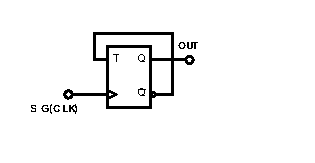
\includegraphics[height=1in]{image/Clock-Edge.pdf}
                \caption{Clock Edge}
                \label{fig:clockEdge}
            \end{figure}
            Another example of using D flip-flop is Clock Edge, as in Figur~\ref{fig:clockEdge}. The effect of it is simple. When clock is reasing from low to high, the output $Q$ is same as the input $D$, otherwise it holds. Thus we see that if we connect $\bar Q$ to $D$, than the output $Q$ will give a clock with double the period.
        \subsubsection{Debounce}
            \begin{figure}[h]
                \centering
                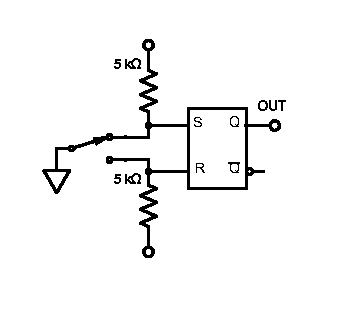
\includegraphics[height=1.3in]{image/Debouncer.pdf}
                \caption{A Debouncer Example}
                \label{fig:debouncer}
            \end{figure}
            Another nice application is a debouncer, as presented in Figur~\ref{fig:debouncer}. This use the hold function so that the output not mistakenly change the output for counter.
\section{Data and Calculation}
    \subsection{Clocks}
        \begin{figure}[h]
            \centering
            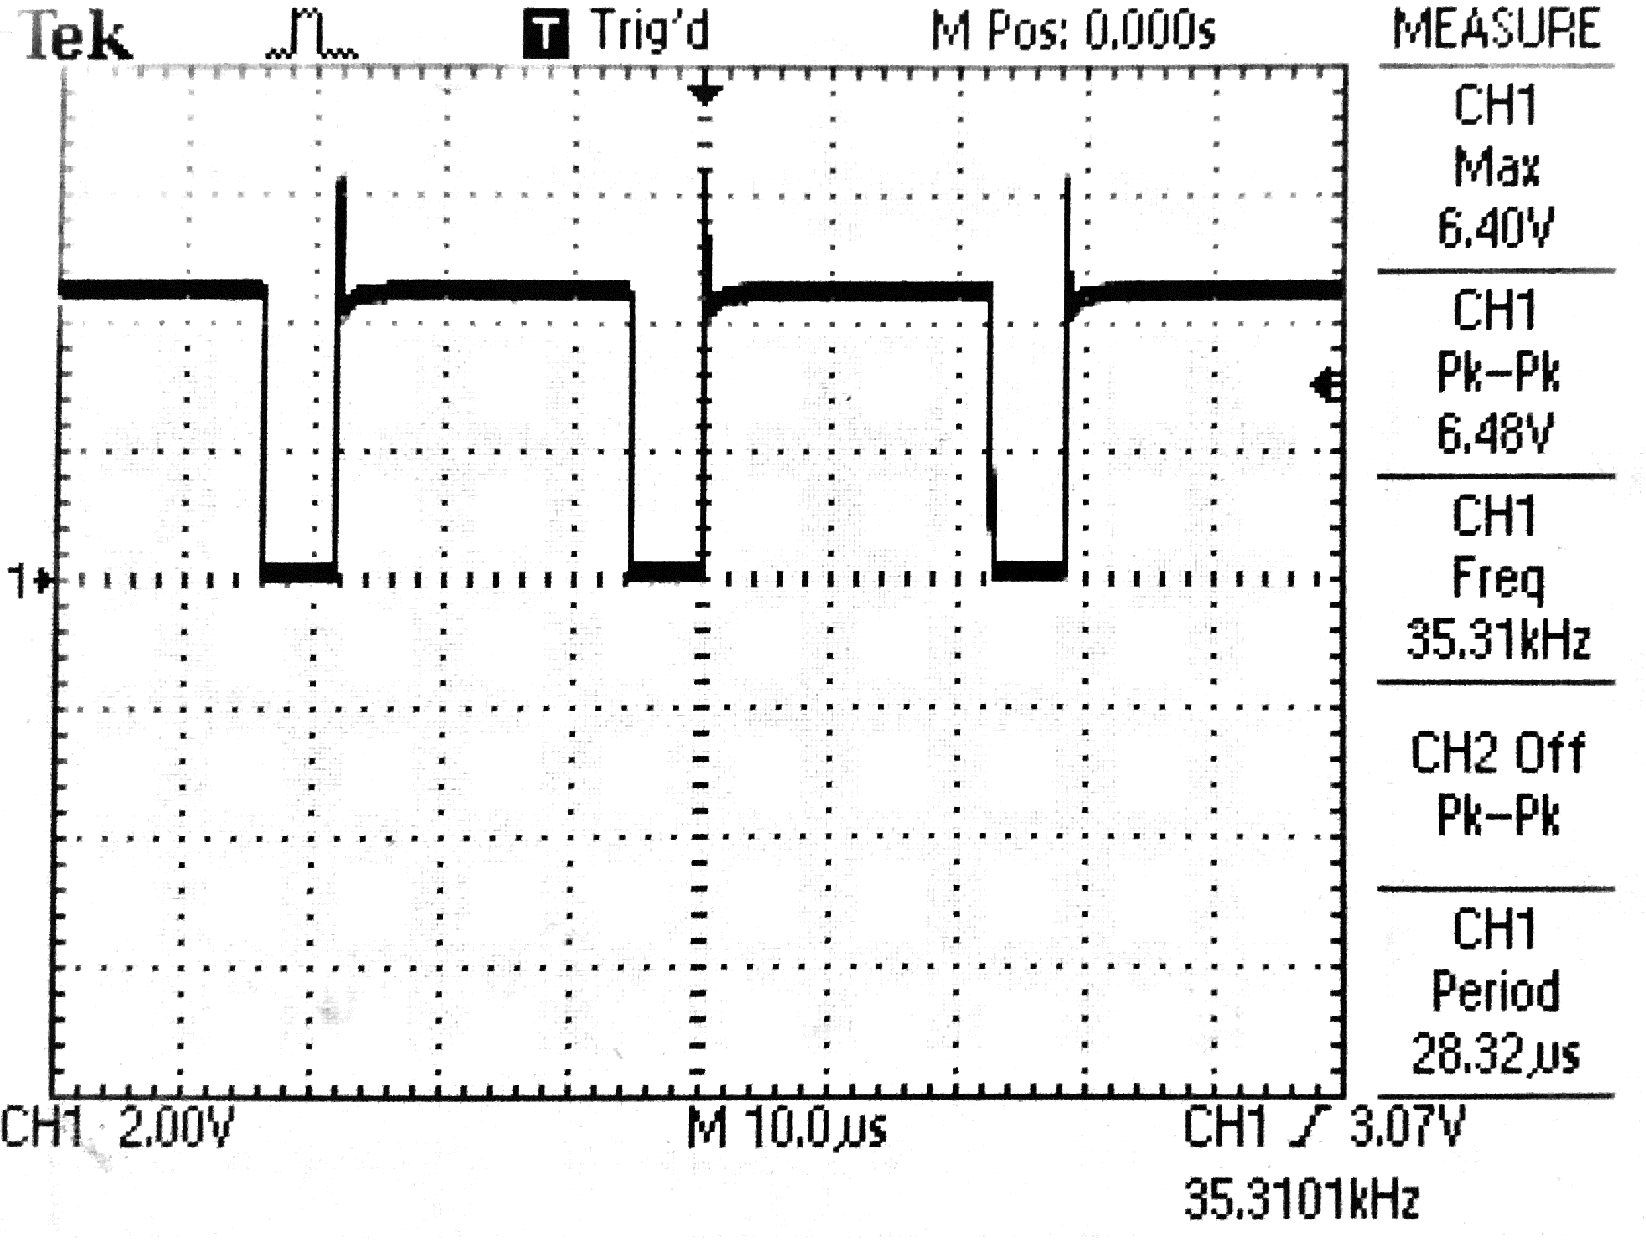
\includegraphics[height=2in]{image/clock-lab.pdf}
            \caption{Result for clock}
            \label{fig:clockResult}
        \end{figure}
        In the lab, we wish to obtain a frequency of 40 kHz and a duty cycle of 80\%. By using Equation~\ref{fig:clocks}, we find $R_1 = 21640\Omega$ and $R_2 = 7213\Omega$ if we want to use a 1nF capastor. In lab, we use a 20.73(2)k$\Omega$ and 7.19(1)k$\Omega$ resistor and a 1.00(1)nF capastor, as shown in Figure~\ref{fig:clocks}.
    \subsection{Signal Generator}
        The signal generator on TTL mode can only give square wave. This wave does not change on high frequency.

    \subsection{XOR gate}
        We want to build a XOR gate using NAND gate, as in Figure~\ref{fig:nandToXor}. The result is same as the truth table of XOR gate.

    \subsection{Two Bit Half-adder}
        Following Figure~\ref{fig:twoBitHalfAdder}, we obtained a two bit half-adder. The result is same as the truth table of a two bit half-adder.

    \subsection{Threshold Test}
        \begin{figure}[h]
            \centering
            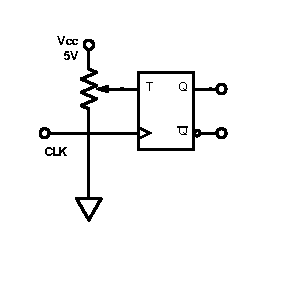
\includegraphics[height=2in]{image/Threshold-Test.pdf}
            \caption{circuit for Threshold Test}
            \label{fig:thresholdTest}
        \end{figure}
        \begin{table}[h]
        \centering
        \begin{tabular}{c c p{0.5in}<{\centering} p{0.5in}<{\centering}} 
        D {[}V{]} & Error on D {[}V{]} & $Q$ & $\bar Q$ \\ \hline\hline
        5.00      & 0.02               & 1 & 0        \\ \hline
        4.95      & 0.02               & 1 & 0        \\ \hline
        4.92      & 0.02               & 1 & 0        \\ \hline
        4.90      & 0.02               & 1 & 0        \\ \hline
        1.7       & 0.02               & 1 & 0        \\ \hline
        1.43      & 0.02               & 1 & 0        \\ \hline
        1.47      & 0.02               & 0 & 1        \\ \hline
        \end{tabular}
        \caption{Result of threshold test}
        \label{tb:threshold}
        \end{table}
        We using the circuit as in Figure~\ref{fig:thresholdTest}. By changing the input voltage, we obtained a result as in Table~\ref{tb:threshold}.
    \subsection{Clock Edge}
        \begin{figure}[h]
            \centering
            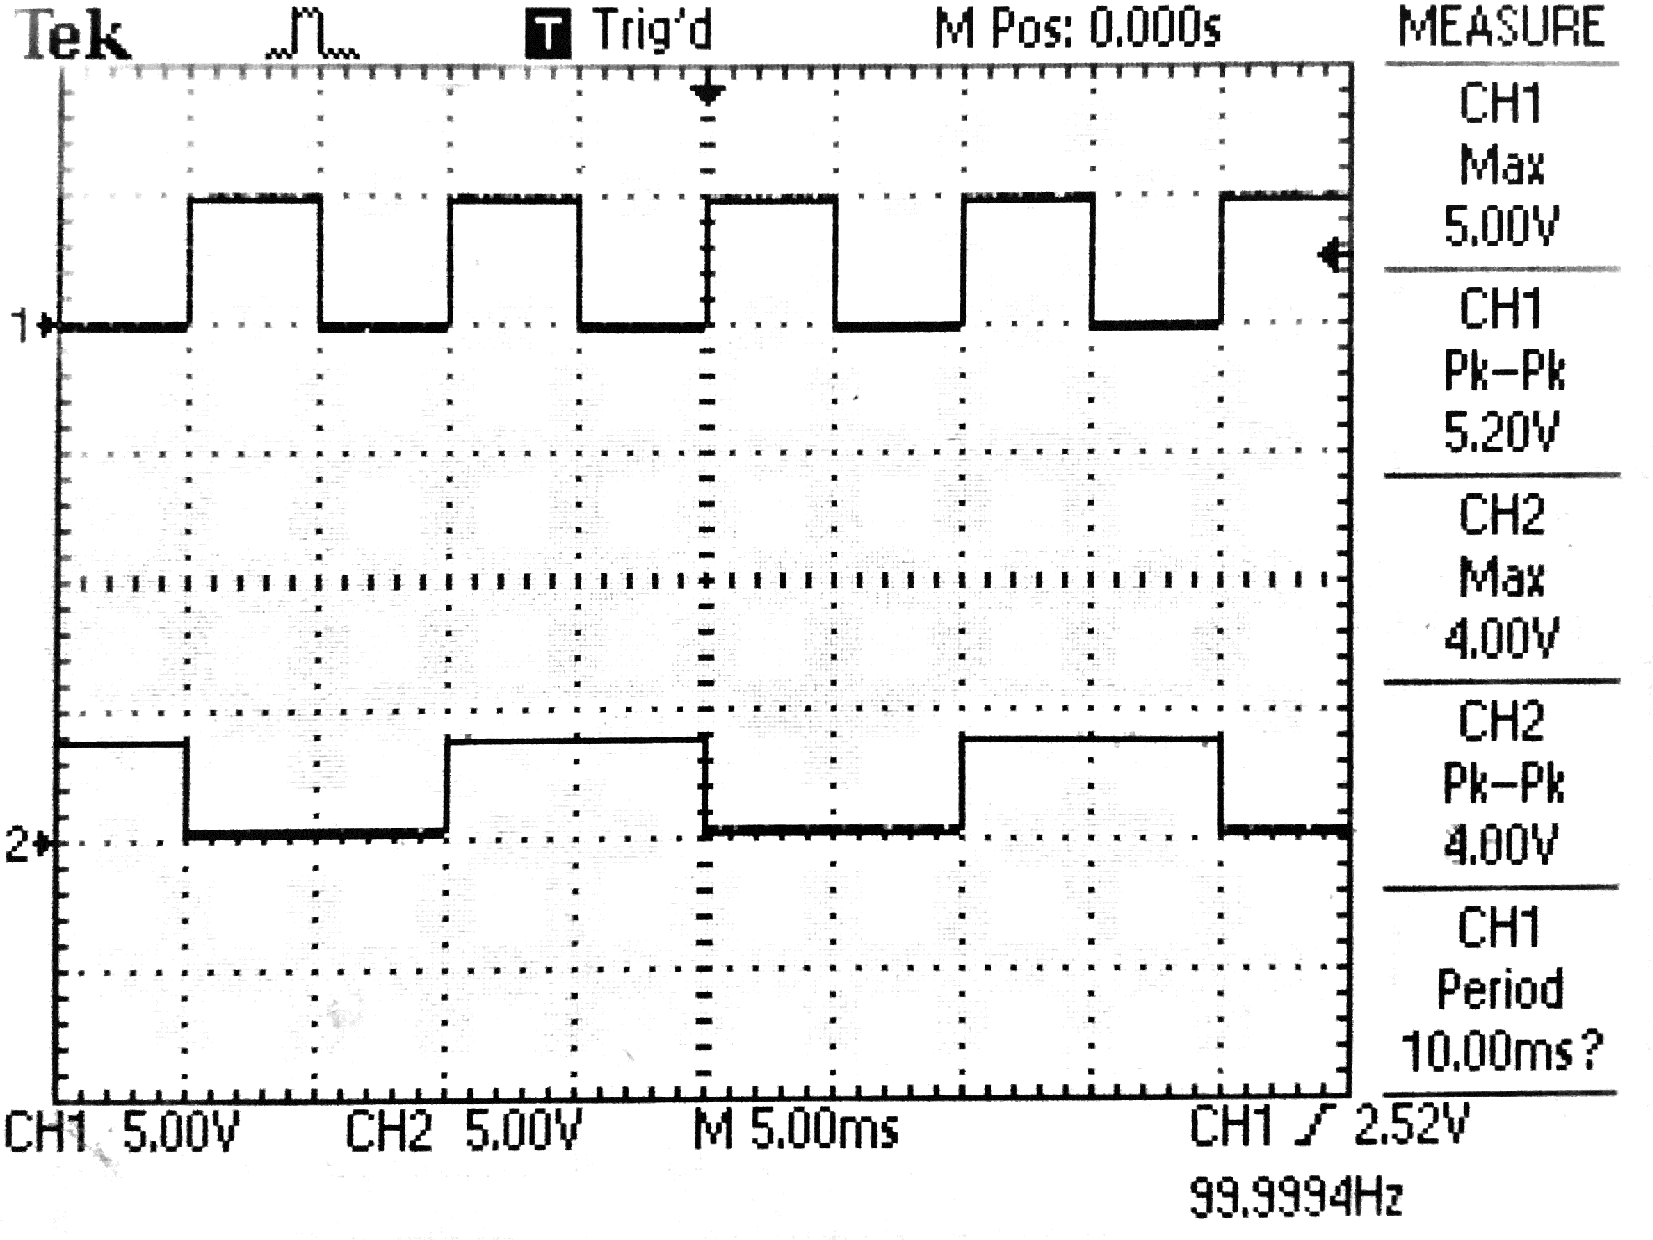
\includegraphics[height=2in]{image/clock-edge-lab.pdf}
            \caption{Result of clock edge}
            \label{fig:clockEdgeLab}
        \end{figure}
        Using a circuit as in Figure~\ref{fig:clockEdge}, we obtained a result as in Figure~\ref{fig:clockEdgeLab}.
    \subsection{Propagation Delay}
        \begin{figure}[h]
            \centering
            \subcaptionbox{Delay for a D flip-flop}[.49\linewidth][c]{%
                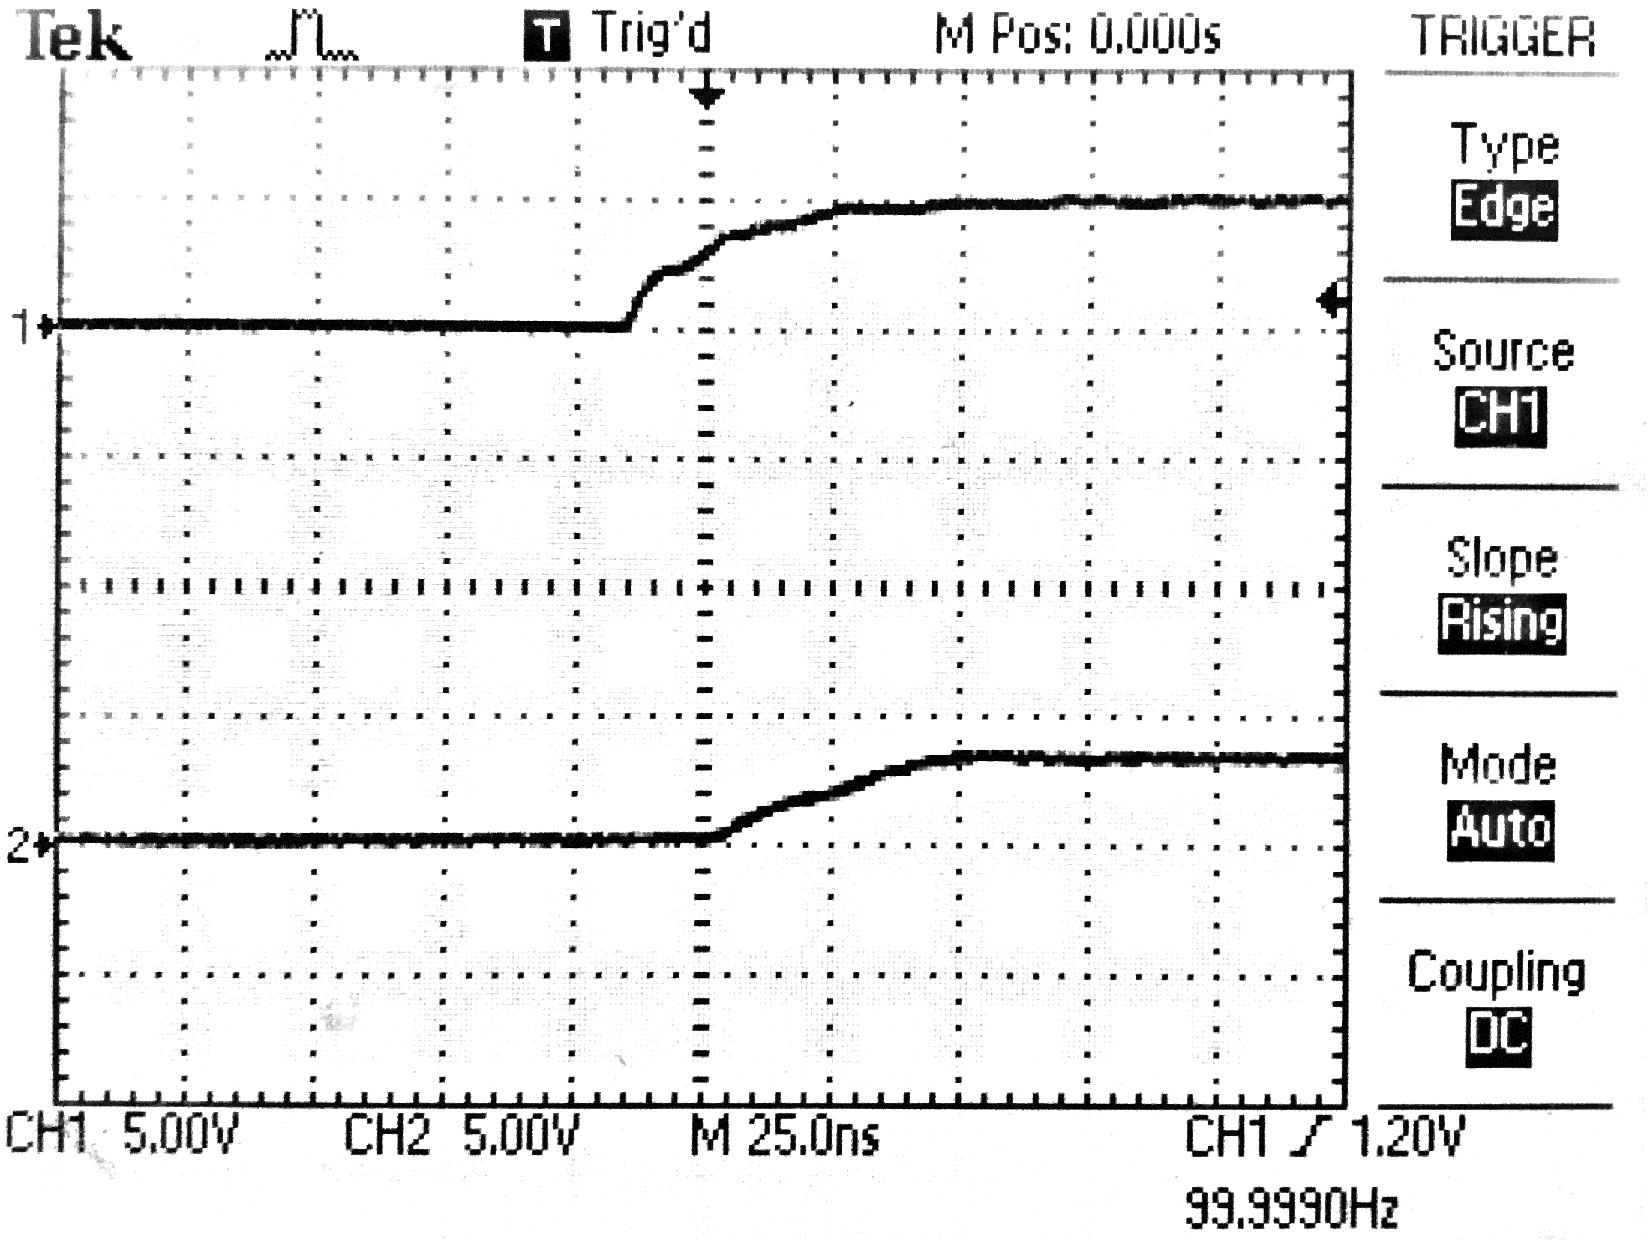
\includegraphics[width=.49\linewidth]{image/delay1.pdf}}
            \subcaptionbox{Delay for a 7404 chip}[.49\linewidth][c]{%
                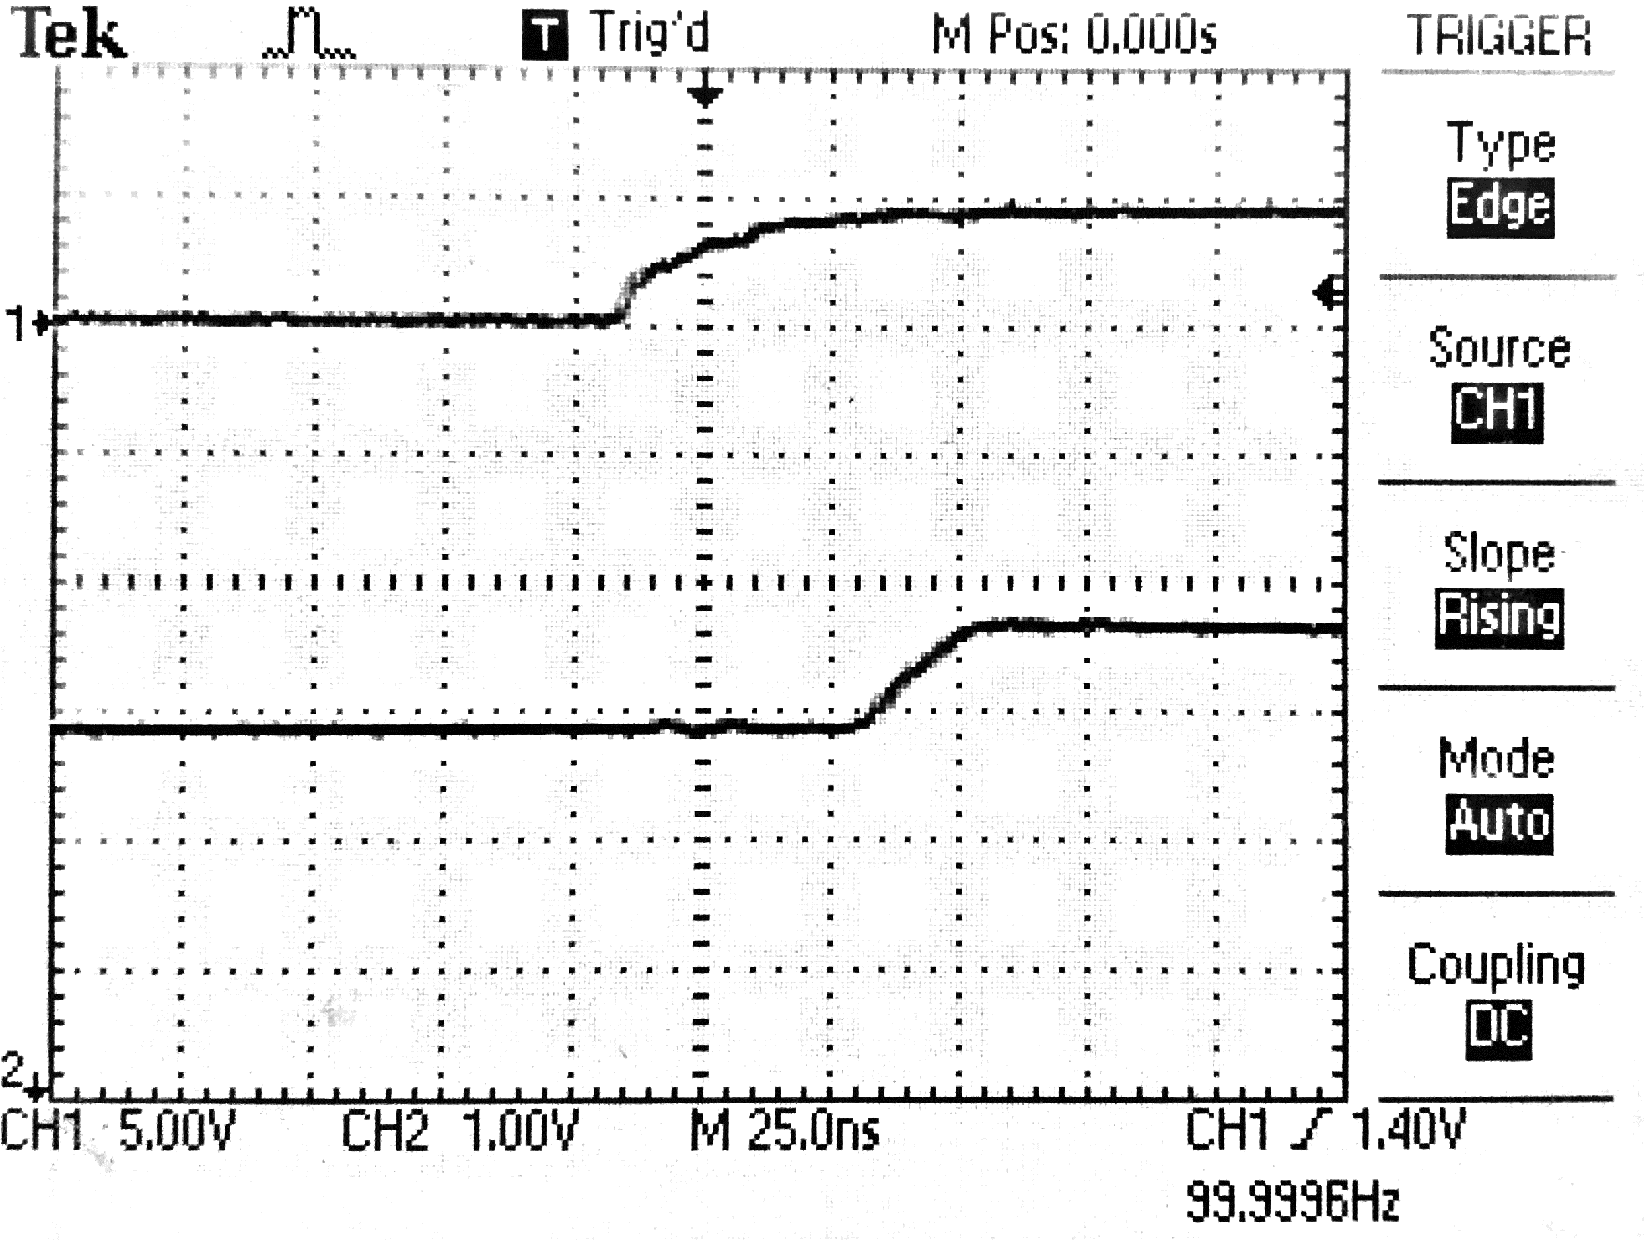
\includegraphics[width=.49\linewidth]{image/delay2.pdf}}
            \caption{Measure Propagatio{}n Dela}
            \label{fig:delay}
        \end{figure}
        Using the clock edge circuit, one can measure the propagation delay of the flip-flop chip. A result is obtained in Figure~\ref{fig:delay}. On the other hand, as a comparison, we also measure a delay of a 7404 chip. We see that the delay of a D flip-flop chip is 15(2)ns. On the other hand, the delay of a 7494 chip is 50(5)ns, which means each component is 8(5)ns.
    \subsection{Debouncer}
        \begin{figure}[h]
            \centering
            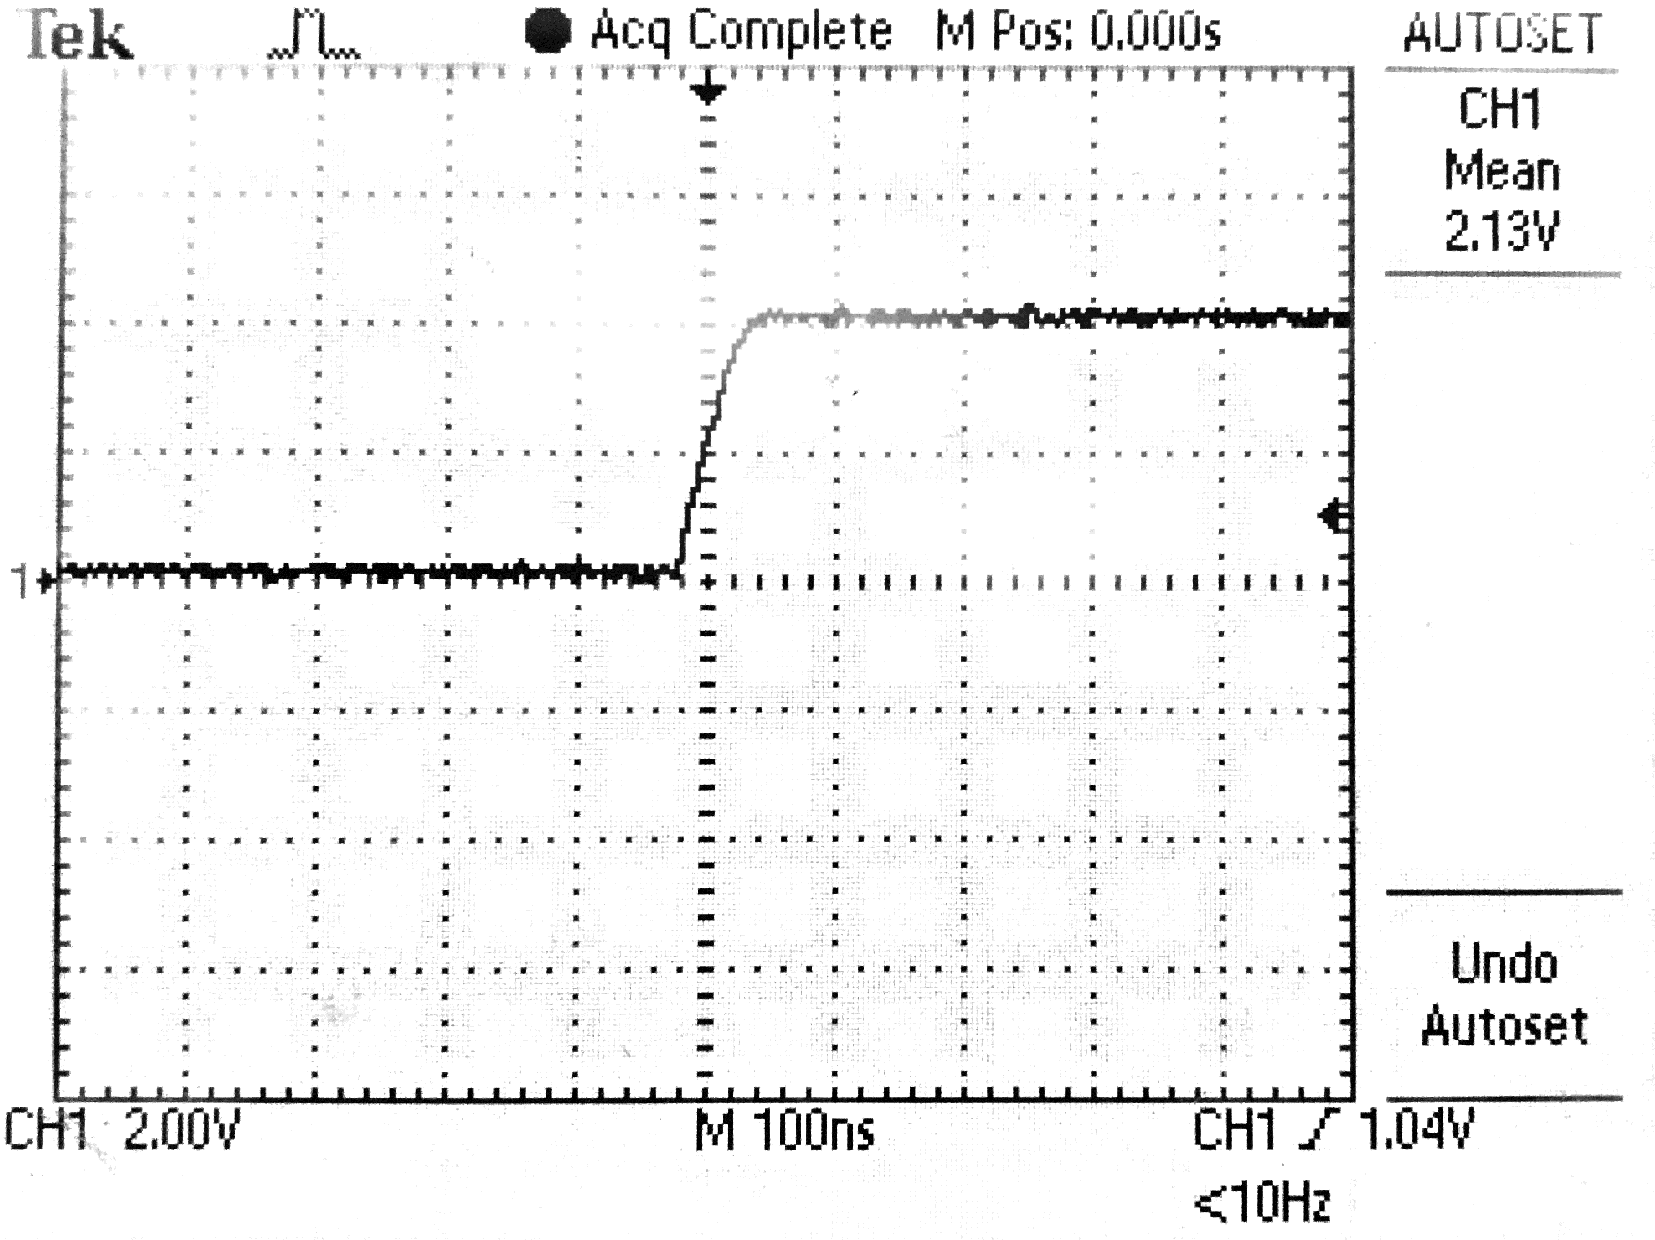
\includegraphics[height=2in]{image/debouncer-lab.pdf}
            \caption{Result of debouncer}
            \label{fig:debouncerLab}
        \end{figure}
        Following Figure~\ref{fig:debouncer}, we can obtained a debouncer. The result of the debouncer is shown as in Figur~\ref{fig:debouncerLab}. We see that the voltage use 60(10)ns from low to high. Indeed, in the lab we see that the output shows the same behavior. By connect the debouncer to a 74393 chip, we obtained a counter of switch press.
\section{Analysis}
    \subsection{Clock}
        From the result we see that we achieve a 35.3(2)kHz clock, it is within a 15\% range of a 40kHz clock. We see that it is a 79(1)\% duty cycle. This result is good.
    \subsection{Signal Generator}
        From the lab we see that signal generator can give a square wave in TTL mode. The wave is independent from the frequency.
    \subsection{XOR Gate}
        In the lab, we successfully achieve a XOR gate by using NAND gate.
    \subsection{Two bit half-adder}
        In the lab, we successfully achieve a two bit half-adder.
    \subsection{Threshold Test}
        From the Table~\ref{tb:threshold}, we see that the output of $Q$ and $\bar Q$ changed at 1.45(2)V. This agree with the TTL standard.
    \subsection{Clock Edge}
        From Figure~\ref{fig:clockEdgeLab}, we see that the output change in the rising edge. We see that the propagation delay of clock edge is lower than the 7404 chip.
    \subsection{Debounce}
        A debouncer have indeed been achieved in the lab. With counter, the circuit behavior properly.

\section{Conclusion}
    The result of this lab is good. One can use a more precise resistor as calculation to achieve a better result on the clock.



\bibliography{cite}
\bibliographystyle{apsrev4-1}

    % \begin{figure}[h]
    %     \centering
    %     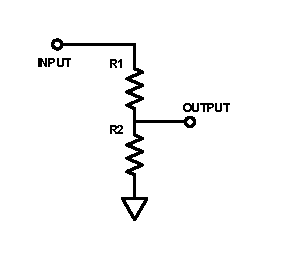
\includegraphics{images/plot2.pdf}
    %     \caption{A voltage divider}
    %     \label{fig:2}
    % \end{figure}

    % \begin{table}[h]
    % \begin{ruledtabular}
    % \begin{tabular}{cccc} 
    % Load[k$\Omega$] &  Output Voltage[V] & $R_\text{th}[\Omega]$ & Theoretical Voltage\\ \hline\hline
    % 50              & 0.680(1)           & 501(1)                & 0.682 \\ \hline
    % 500             & 3.75(1)            & 500(1)                & 3.75 \\ \hline
    % 5000            & 6.80(1)            & 514(1)                & 6.82 \\
    % \end{tabular}
    % \end{ruledtabular}
    % \caption{Load resistor and the output}
    % \label{table:8}
    % \end{table} 

% \begin{center}
%  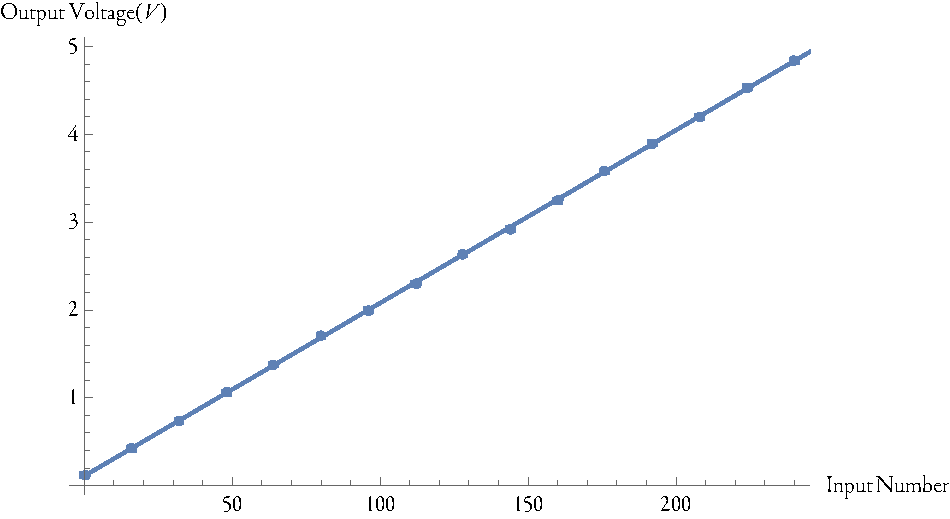
\includegraphics[height=1.8in]{plot.pdf}
% \end{center} 

%\begin{center}
% 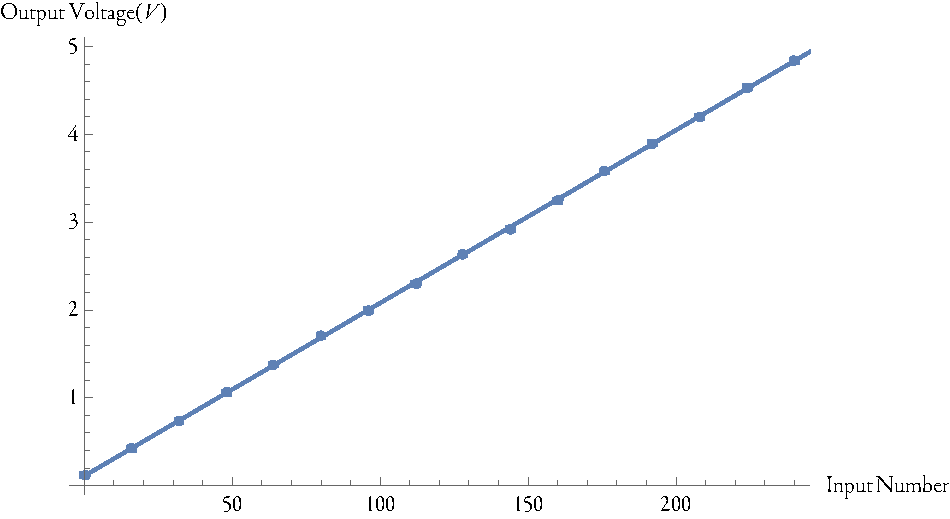
\includegraphics[height=1.3in]{plot.pdf}
%\end{center}

% \blindtext \cite{article-minimal}

% \bibliographystyle{apsrev4-1} % Tell bibtex which bibliography style to use
% \bibliography{xampl} % Tell bibtex which .bib file to use (this one is some example file in TexLive's file tree)

\end{document}